\documentclass[a4paper]{article}
\usepackage[utf8]{inputenc}
\usepackage[T1]{fontenc}
\usepackage[pdftex]{graphicx}
\usepackage{fancyhdr}
\usepackage{lscape}
\usepackage{color}
\usepackage{qtree}
\usepackage[english]{babel}
\usepackage{graphicx}
\usepackage[colorinlistoftodos]{todonotes}
\usepackage{listings}
\usepackage{color}
\usepackage{float}
\usepackage{changepage}
\usepackage[margin=1in]{geometry}
\definecolor{codegreen}{rgb}{0,0.6,0}
\definecolor{codegray}{rgb}{0.5,0.5,0.5}
\definecolor{codepurple}{rgb}{0.58,0,0.82}
\definecolor{backcolour}{rgb}{0.95,0.95,0.92}
\usepackage[final]{pdfpages} 
 
 \lstdefinestyle{mystyle}{
 	backgroundcolor=\color{backcolour},   
 	commentstyle=\color{codegreen},
 	keywordstyle=\color{magenta},
 	numberstyle=\tiny\color{codegray},
 	stringstyle=\color{codepurple},
 	basicstyle=\footnotesize,
 	breakatwhitespace=false,         
 	breaklines=true,                 
 	captionpos=b,                    
 	keepspaces=true,                 
 	numbers=left,                    
 	numbersep=5pt,                  
 	showspaces=false,                
 	showstringspaces=false,
 	showtabs=false,                  
 	tabsize=2
 }
 
\lstset{
	style=mystyle,
	inputencoding=utf8,
	extendedchars=true,
	literate={á}{{\'a}}1 {ã}{{\~a}}1 {é}{{\'e}}1,
	escapechar=\&
}
\title{Algorithmique et structures de données : Mission 3 correction croisée}

\author{Groupe 1.2: Ivan Ahad - Jérôme Bertaux - Rodolphe Cambier \\ 
	Baptiste Degryse - Wojciech Grynczel - Charles Jaquet}

\begin{document}

\section*{Performance}
Pour analyser les performances du tri, j'ai dû modifier le programme pour lui permettre de faire des dictionnaires avec un nombre d'éléments prédéfini. Ensuite j'ai fait les calculs du temps moyens pour créer une liste triée des éléments. Enfin j'ai écris ces temps dans un fichier qui m'a permet de tracer le graphe (fig. \ref{perfo}) du temps nécéssaire pour créer une liste ordonnée en partant de la treeMap en fonction du nombre d'éléments.


\begin{figure} [h!]
\begin{center}
\includegraphics[scale=0.4]{performanceListeOrdonnee.eps}
\caption{Graphe du temps pour créer une liste ordonnée en partant du TreeMap en fonction du nombre d'éléments}
\label{perfo}
\end{center}
\end{figure}

Ensuite, en fonction du nombre d'éléments, nous avons calculé le temps pris pour trouver un élément dans la liste. (Fig. \ref{perfoFind})

\begin{figure} [h!]
\begin{center}
\includegraphics[scale=0.4]{performanceFind.eps}
\caption{Temps moyen mis pour trouvé un élément}
\label{perfoFind}
\end{center}
\end{figure}

Etonnement, nous avons un temps stable or que nous nous attendions à ce que ça évolue de manière logarithmique

\end{document}
